\newpage
\chapter{Въвеждане на данни и извеждане на графики}
\label{chapter04}
\thispagestyle{empty}

Статистическата обработка на данни в R започва с въвеждането на събраната информация\index{въвеждане на информация} и завършва с визуализация на резултатите\index{визуализация на резултатите} от анализа. Тези две фази от етапа на статистическата обработка имат своята важност, тъй като входните данни силно определят надеждността на извършвания анализ, а правилно визуализираните резултати определят степента на разбиране, която ще постигне аудиторията, пред която анализът се представя.

\section{Въвеждане на данни от външни източници}

Данните в примерите до тази глава бяха фиксирани и се въвеждаха ръчно от конзолата, в интерактивен режим. Този начин на работа не е най-рационалния, когато се правят модели и с данните за модела се провеждат многократни експерименти. Обичайната практика е командите за съставянето на модела да бъдат написани в обикновен текстов файл, с разширение „.r“, а данните да бъдат зареждани от външен файл\index{четене от файл}. Този начин на работа позволява да бъдат създадени множество модели, които често се различават по нещо дребно и също да бъдат зареждани различни входни данни, например за различни периоди на измерване.

\subsection{CSV файлове}

Продуктът R позволява множество различни начини за въвеждане на данни в системата, но най-достъпният начин е през CSV (Comma Separated Values) файлове. CSV файловият формат е текстов файлов формат, който позволява таблично представяне на данни (колони и редове). CSV може да бъде четен и редактиран с обикновен текстов редактор, като Notepad под Microsoft Windows, TextEdit под Mac OS X или Nano под Linux. CSV комфортно се визуализира и обработва от продуктите Microsoft Excel, OpenOffice Calc и Libre Calc.

\begin{lstlisting}[caption=Зареждане на данни от CSV файл, label=listing0053]
df <- read.table(file="http://raw.githubusercontent.com/TodorBalabanov/Statistical-Data-Processing-with-R/master/data/tomato.csv", header=TRUE, sep=",")

head( df )
  Round             Tomato Price      Source Sweet Acid Color Texture Overall
1     1         Simpson SM  3.99 Whole Foods   2.8  2.8   3.7     3.4     3.4
2     1  Tuttorosso (blue)  2.99     Pioneer   3.3  2.8   3.4     3.0     2.9
3     1 Tuttorosso (green)  0.99     Pioneer   2.8  2.6   3.3     2.8     2.9
4     1     La Fede SM DOP  3.99   Shop Rite   2.6  2.8   3.0     2.3     2.8
5     2       Cento SM DOP  5.49  D Agostino   3.3  3.1   2.9     2.8     3.1
6     2      Cento Organic  4.99  D Agostino   3.2  2.9   2.9     3.1     2.9
  Avg.of.Totals Total.of.Avg
1          16.1         16.1
2          15.3         15.3
3          14.3         14.3
4          13.4         13.4
5          14.4         15.2
6          15.5         15.1

tail( df )
   Round                   Tomato Price      Source Sweet Acid Color Texture
11     3       Scotts Backyard SM  0.00  Home Grown   1.6  2.9   3.1     2.4
12     3 Di Casa Barone (organic) 12.80      Eataly   1.7  3.6   3.8     2.3
13     4         Trader Joes Plum  1.49 Trader Joes   3.4  3.3   4.0     3.6
14     4          365 Whole Foods  1.49 Whole Foods   2.8  2.7   3.4     3.1
15     4        Muir Glen Organic  3.19 Whole Foods   2.9  2.8   2.7     3.2
16     4        Bionature Organic  3.39 Whole Foods   2.4  3.3   3.4     3.2
   Overall Avg.of.Totals Total.of.Avg
11     1.9          11.9         11.9
12     1.4          12.7         12.7
13     3.9          17.8         18.2
14     3.1          14.8         15.2
15     3.1          14.8         14.7
16     2.8          15.1         15.2
\end{lstlisting}

Зареждането на CSV в R най-ефективно се постига с функцията read.table (Листинг \ref{listing0053}). Резултатът от четенето е обект от тип рамкирани данни. При извикването на функцията, параметрите се подават с явно изписване на имената им. Точният адрес на файла се подава в кавички, а когато първият ред от данните е заглавен ред, се подава флаг за заглавен ред. Третият аргумент е за указване на разделителя в редовете, тъй като не винаги този разделител е запетая. Често софтуерните продукти за електронни таблици поставят символа за табулация като разделител между данните на един ред. Символът табулация попада в групата на белите символи (white spaces), тъй като не се изобразява видимо, а с празно пространство. Когато трябва да бъде подаден като аргумент, за разделител се използва комбинацията от обратна наклонена черта и буквата t (\textbackslash t).

\begin{lstlisting}[caption=Проверка на типовете\, които колоните имат, label=listing0054]
sapply(df, class)
        Round        Tomato         Price        Source         Sweet 
    "integer"      "factor"     "numeric"      "factor"     "numeric" 
         Acid         Color       Texture       Overall Avg.of.Totals 
    "numeric"     "numeric"     "numeric"     "numeric"     "numeric" 
 Total.of.Avg 
    "numeric" 
\end{lstlisting}

При зареждане на данни от CSV файл по подразбиране текстовите колони се зареждат като фактори\index{фактори}, а не като вектори от символни низове (Листинг \ref{listing0054}). Тъй като използването на фактори има своите особености, понякога се налага зареждането да става в символни низове. За тези случаи функцията read.table има параметър stringsAsFactors, който може да се установи на FALSE и това ще предотврати зареждането на фактори (Листинг \ref{listing0055}).

\begin{lstlisting}[caption=Зареждане на символни низове, label=listing0055]
sapply(read.table(file="http://raw.githubusercontent.com/TodorBalabanov/Statistical-Data-Processing-with-R/master/data/tomato.csv", header=TRUE, sep=",", stringsAsFactors=FALSE), class)
        Round        Tomato         Price        Source         Sweet 
    "integer"   "character"     "numeric"   "character"     "numeric" 
         Acid         Color       Texture       Overall Avg.of.Totals 
    "numeric"     "numeric"     "numeric"     "numeric"     "numeric" 
 Total.of.Avg 
    "numeric"
\end{lstlisting}

Същият аргумент може да се използва и във функцията data.frame, когато от вектори се създават рамкирани данни.

Възможно е да се появят проблеми с прочитането на CSV файловете. Причини за тези проблеми може да са лошо форматиране или наличие на разделители за стойностите в редовете. В такива ситуации могат да се пробват алтернативните функциите за четене, каквито са $read.csv2$ и $read.delim2$.

\subsection{Excel файлове}

Microsoft Excel\index{електронни таблици} е може би най-популярният инструмент за извършване на статистически анализи и въпреки това четенето на Excel файлове в R не е толкова лесно. Основните трудности идват от това, че Microsoft Excel е комерсиален софтуер и бинарните му файлови формати не са с отворен лиценз. Най-лесният начин за четене на данни от Excel е файловете да бъдат съхранени като CSV файлове.

Общността разработчици полага някои усилия да осигури четене на Excel файлове директно в R, но наличните пакети, като gdata, XLConnect, xlsReadWrite, далеч не са достатъчно надеждни и често изискват допълнителни софтуерни модули, като Java, Perl или 32 битова версия на R. В пакета RODBC съществува функция odbcConnectExcel2007, която чете Excel файлове, но тя изисква DSN (Data Source Name) връзка (най-често връзка към база данни). По своята структура, файловете след Excel 2007 са в XML формат, което би трябвало да улеснява разчитането им, но за момента R не предлага такава възможност.

\subsection{SQL бази данни}

Голямо количество от данните, събирани до наши дни, се съхраняват в бази данни\index{бази данни}. Повечето от тези системи за управление на бази от данни са релационни и разчитат на езика SQL \cite{sql} за манипулация на структурата или самите данни. За най-популярните релационни бази данни в R са достъпни пакети като RpostgreSQL или RmySQL. За други релационни бази данни, които не са съпровождани с конкретен R пакет може да се използва пакетът RODBC. Връзката към база данни може да е съпроводена с много трудности и поради тази причина е създаден пакетът DBI. Този пакет позволява унифициран начин на работа с различните бази данни.

Боравенето с релационна база данни е извън обхвата на настоящото изложение и вследствие на тази причина примерите са реализирани на SQLite като една от най-достъпните и лесни за използване системи за управление на бази от данни.

Командният интерпретатор на R се изпълнява с конкретна работна директория. С функцията getwd тази директория може да бъде проверена, а с функцията setwd директорията може да бъде променена (Листинг \ref{listing0056}).

\begin{lstlisting}[caption=Работна директория, label=listing0056]
getwd()
[1] "/Users/todorbalabanov"

setwd("~/Desktop")
getwd()
[1] "/Users/todorbalabanov/Desktop"
\end{lstlisting}

За улеснение по време на работа, работната директория се установява да бъде директорията на работния плот, където ще се разположи и файлът с данните. Файлът може да бъде свален и със средствата на операционната система, но R предоставя команда за тази операция (Листинг \ref{listing0057}).

\begin{lstlisting}[caption=Сваляне на файл с данни, label=listing0057]
download.file("https://github.com/TodorBalabanov/Statistical-Data-Processing-with-R/blob/master/data/diamonds.db?raw=true", destfile="./diamonds.db", mode="wb")

trying URL 'https://github.com/TodorBalabanov/Statistical-Data-Processing-with-R/blob/master/data/diamonds.db?raw=true'

Content type 'application/octet-stream' length 5909504 bytes (5.6 MB)
==================================================
downloaded 5.6 MB
\end{lstlisting}

Едно от многото предимства на SQLite е, че базата данни се помества в един единствен файл. Тъй като за SQLite е разработен конкретен R пакет, то той се използва за връзка с данните (Листинг \ref{listing0058}). При липса на конкретен пакет остава алтернативата за използване на RODBC.

\begin{lstlisting}[caption=Връзка към базата данни, label=listing0058]
library(RSQLite)

driver <- dbDriver( "SQLite" )
class( driver )
[1] "SQLiteDriver"
attr(,"package")
[1] "RSQLite"

connection <- dbConnect(driver, "./diamonds.db")
class( connection )
[1] "SQLiteConnection"
attr(,"package")
[1] "RSQLite"
\end{lstlisting}

След зареждането на пакета за работа с базата данни се зарежда драйверът. Променливата, която съдържа драйвера се подава като аргумент на функцията за осъществяване на връзка към базата данни. Командата за осъществяване на връзка към базата данни може да се различава за различните операционни системи, така че е съществено да се провери документацията на R за конкретната операционна система.

След като бъде изградена връзка към базата данни, може да се изпълнят команди за изследване на структурата и данните (Листинг \ref{listing0059}).

\begin{lstlisting}[caption=Изследване на базата данни, label=listing0059]
dbListTables( connection )
[1] "DiamondColors" "diamonds"      "sqlite_stat1" 

dbListFields(connection, name="diamonds")
 [1] "carat"   "cut"     "color"   "clarity" "depth"   "table"   "price"  
 [8] "x"       "y"       "z"

dbListFields(connection, name="DiamondColors")
[1] "Color"       "Description" "Details"
\end{lstlisting}

Когато структурата на базата данни е известна, над нея могат да се изпълняват всички валидни SQL заявки. Тази цел се постига с функцията dbGetQuery, която връща data.frame структура в резултат (Листинг \ref{listing0060}).

\begin{lstlisting}[caption=Изследване на базата данни, label=listing0060]
# Simple select query.
diamondsTable <- dbGetQuery(connection, "SELECT * FROM diamonds", stringsAsFactors = FALSE)
colorTable <- dbGetQuery(connection, "SELECT * FROM DiamondColors", stringsAsFactors = FALSE)

# Join between the two tables.
diamondsJoin <-dbGetQuery(connection, "SELECT * FROM diamonds, DiamondColors WHERE diamonds.color = DiamondColors.Color", stringsAsFactors = FALSE)

head(diamondsTable, n=3)
  carat     cut color clarity depth table price    x    y    z
1  0.23   Ideal     E     SI2  61.5    55   326 3.95 3.98 2.43
2  0.21 Premium     E     SI1  59.8    61   326 3.89 3.84 2.31
3  0.23    Good     E     VS1  56.9    65   327 4.05 4.07 2.31
 
head(colorTable, n=3)
  Color          Description                Details
1     D Absolutely Colorless               No color
2     E            Colorless Minute traces of color
3     F            Colorless Minute traces of color

head(diamondsJoin, n=3)
  carat     cut color clarity depth table price    x    y    z Color
1  0.23   Ideal     E     SI2  61.5    55   326 3.95 3.98 2.43     E
2  0.21 Premium     E     SI1  59.8    61   326 3.89 3.84 2.31     E
3  0.23    Good     E     VS1  56.9    65   327 4.05 4.07 2.31     E
  Description                Details
1   Colorless Minute traces of color
2   Colorless Minute traces of color
3   Colorless Minute traces of color
\end{lstlisting}

При затварянето на R сесията, връзката към базата данни ще бъде прекратена, но добрата работна практика изисква всички ненужни повече ресурси да се освобождават веднага, след като работата с тях приключи. За тази цел в R има команда за прекратяване на връзката към базата данни (Листинг \ref{listing0061}).

\begin{lstlisting}[caption=Прекъсване на връзката към базата данни, label=listing0061]
dbDisconnect( connection )
\end{lstlisting}

Важно е също да се вземе предвид, че R може да поддържа само една връзка към база данни в конкретен период от време. При нужда да се работи с повече от една база данни, връзките трябва да се редуват.

\subsection{Други статистически програми като източници на данни}

Тъй като R е само една от алтернативите за статистическа обработка на данни, в реалната практика се използват множество други софтуерни решения, част от които разчитат на затворени (търговски) файлови формати\index{файлови формати} (например SPSS, SAS или Octave). За достъп до тези файлове, пакетът foreign предлага множество функции, работещи по сходен начин на функцията read.table. Част от функциите са изброени в Таблица \ref{table0001}.

\begin{table}[h!]
\centering
\begin{tabular}{|l|r|} 
  \rowcolor{lightgray}
  \hline
  Функция & Файлов формат \\ [0.1ex] 
  \hline\hline
  read.spss & SPSS \\
  \hline
  read.ssd & SAS \\
  \hline
  read.ocatave & Octave \\
  \hline
  read.dta & Stata \\
  \hline
  read.systat & Systat \\
  \hline
  read.mtp & Minitab \\
  \hline
\end{tabular}
\caption{Функции за четене на данни}
\label{table0001}
\end{table}

Параметрите на групата функции са подобни на параметрите подавани към read.table. В общия случай, функциите връщат резултат под формата на data.frame. За някои файлови формати (например SAS) може да се изисква валиден софтуерен лиценз.

\subsection{Бинарни файлове на R}

При работа между различни R потребители е удачно информацията да се разменя в бинарния файлов формат поддържан от R (Rdata)\index{бинарни файлове}. Този файлов формат е бинарен и поддържа различните обекти, които са достъпни в процеса на работа с R. Голямо предимство на този файлов формат е, че е съвместим с различните операционни системи и може да се предават данни между различни инсталации на програмния продукт.

\begin{lstlisting}[caption=Използване на множество от данни, label=listing0062]
tomato <- read.table(file="http://raw.githubusercontent.com/TodorBalabanov/Statistical-Data-Processing-with-R/master/data/tomato.csv", header=TRUE, sep=",")

head(tomato, n=3)
  Round             Tomato Price      Source Sweet Acid Color Texture Overall
1     1         Simpson SM  3.99 Whole Foods   2.8  2.8   3.7     3.4     3.4
2     1  Tuttorosso (blue)  2.99     Pioneer   3.3  2.8   3.4     3.0     2.9
3     1 Tuttorosso (green)  0.99     Pioneer   2.8  2.6   3.3     2.8     2.9
  Avg.of.Totals Total.of.Avg
1          16.1         16.1
2          15.3         15.3
3          14.3         14.3
\end{lstlisting}

При наличен data.frame в общата памет (Листинг \ref{listing0062}), следва да се изпълнят команди за съхраняване, изтриване на общата памет и прочитане на съхранените данни (Листинг \ref{listing0063}).

\begin{lstlisting}[caption=Запис и четене в RData файл, label=listing0063]
save(tomato, file="./tomato.rdata")

rm( tomato )

head( tomato )
Error in head(tomato) : object 'tomato' not found

load("tomato.rdata")

head(tomato, n=3)
  Round             Tomato Price      Source Sweet Acid Color Texture Overall
1     1         Simpson SM  3.99 Whole Foods   2.8  2.8   3.7     3.4     3.4
2     1  Tuttorosso (blue)  2.99     Pioneer   3.3  2.8   3.4     3.0     2.9
3     1 Tuttorosso (green)  0.99     Pioneer   2.8  2.6   3.3     2.8     2.9
  Avg.of.Totals Total.of.Avg
1          16.1         16.1
2          15.3         15.3
3          14.3         14.3
\end{lstlisting}

Всички обекти, които трябва да се съхранят в RData файла се изброяват преди името на самия файл. При възстановяването им от диска в общата памет те придобиват имената, които са имали по време на съхраняването.

\begin{lstlisting}[caption=Запис и четене на един обект, label=listing0064]
saveRDS(c(21,04,1979), "object.rds")

readRDS("object.rds")
[1]   21    4 1979
\end{lstlisting}

Съществува и втора възможност за запазване на данни, под формата на RDS файл. Запазването става с функцията saveRDS\index{съхраняване на обект}, а прочитането с функцията readRDS\index{зареждане на обект}. Разликата с предходните функции е, че в този случай се съхранява само един обект, без да се запазва неговото име и при прочитането резултатът трябва да се присвои изрично на променлива (Листинг \ref{listing0064}).

\subsection{Данни достъпни директно от R}

Софтуерният продукт R и някои от неговите пакети идват с предварително заложени множества от данни\index{демонстрационни данни}. Този вид примерни данни основно се използват за демонстриране на възможностите, които R има или възможностите, които съответният пакет предоставя. За да бъдат ползвани тези данни е достатъчно да се знае в кой пакет се намират.

\begin{lstlisting}[caption=Зареждане на примерни данни, label=listing0065]
data(diamonds, package="ggplot2")

head(diamonds, n=3)
  carat     cut color clarity depth table price    x    y    z
1  0.23   Ideal     E     SI2  61.5    55   326 3.95 3.98 2.43
2  0.21 Premium     E     SI1  59.8    61   326 3.89 3.84 2.31
3  0.23    Good     E     VS1  56.9    65   327 4.05 4.07 2.31
\end{lstlisting}

Зареждането става с функцията data и името на пакета. Като например, множеството данни за диамантите е налично в пакета ggplot2 (Листинг \ref{listing0065}). Списък на всички налични комплекти от данни може да се получи, ако функцията data се извика без аргументи.

\subsection{Четене на данни от JSON формат}

Един от най-популярните съвременни формати на данни е JSON\index{JSON данни} \cite{json}. Първоначално е замислен като формат за обмен на JavaScript обекти, но след това намира широко приложение в множество софтуерни решения. JSON се използва за съхраняване и предаване на структурирана информация в чист текстов вид (plain text). Два са основните пакета за четене на JSON в R (rjson и jsonlite).

\begin{lstlisting}[caption=Четене на JSON данни, label=listing0066]
library( jsonlite )
 
pizza <- fromJSON("https://raw.githubusercontent.com/TodorBalabanov/Statistical-Data-Processing-with-R/master/data/pizza.json")

head(pizza, n=3)
           Name                               Details
1 Di Fara Pizza    1424 Avenue J, Brooklyn, NY, 11230
2 Fiore's Pizza  165 Bleecker St, New York, NY, 10012
3     Juliana's 19 Old Fulton St, Brooklyn, NY, 11201

class( pizza )
[1] "data.frame"
 
class( pizza$Name )
[1] "character"
 
class( pizza$Details )
"list"

class( pizza$Details[[1]] )
[1] "data.frame
\end{lstlisting}

Примерният файл съдържа описание на ресторанти за пица, което включва: име и подробности (адрес, град, пощенски код и телефон). Функцията formJSON (Листинг \ref{listing0066}) се опитва да представи резултата в data.frame структура. Такова представяне не винаги е възможно, тъй като JSON данните могат да бъдат организирани в сложна и/или непълна йерархия. Резултатът от четенето на примерните данни за пица-ресторантите е data.frame в две колони, но по своята същност всеки елемент в Details е също data.frame.

\section{Визуализация на данни от статистически анализ}

Една от най-трудните и отговорни фази в статистическата обработка на данни е визуализацията\index{визуализация на данни} на получените резултати. Доброто графично оформление на получените резултати може значително да подобри разбирането на информацията от аудиторията, пред която тя се представя. За визуално оформление на резултатите, R предоставя достатъчно възможности, както в основната инсталация, така и в допълнителните пакети, като ggplot2 и lattice.

За да се демонстрират графичните възможности на R е необходимо зареждането на подходящо множество от данни. Такова множество от данни е diamonds в пакета ggplot2 (Листинг \ref{listing0067}).

\begin{lstlisting}[caption=Четене на JSON данни, label=listing0067]
library( ggplot2 )

data( diamonds )
 
head(diamonds, n=3)
# A tibble: 3 x 10
  carat cut     color clarity depth table price     x     y     z
  <dbl> <ord>   <ord> <ord>   <dbl> <dbl> <int> <dbl> <dbl> <dbl>
1  0.23 Ideal   E     SI2      61.5    55   326  3.95  3.98  2.43
2  0.21 Premium E     SI1      59.8    61   326  3.89  3.84  2.31
3  0.23 Good    E     VS1      56.9    65   327  4.05  4.07  2.31
\end{lstlisting}

Данните за диамантите са организирани в 10 колони и отчитат 10 различни характеристики на скъпоценните камъни (Таблица \ref{table0002}).

\begin{table}[h!]
\centering
\begin{tabular}{|l|r|} 
  \rowcolor{lightgray}
  \hline
  Характеристика & Значение \\ [0.1ex] 
  \hline\hline
  carat & Тегло на камъка (дробно число) \\
  \hline
  cut & Качество на среза (изброимо множество) \\
  \hline
  color & Цвят на камъка (изброимо множество) \\
  \hline
  clarity & Чистота на камъка (изброимо множество) \\
  \hline
  depth & Дълбочина на камъка (проценти) \\
  \hline
  table & Ширина на горната част, спрямо най-широката част (дробно число) \\
  \hline
  price & Цена (щатски долари) \\
  \hline
  x & Дължина (милиметри) \\
  \hline
  y & Ширина (милиметри) \\
  \hline
  z & Дълбочина (милиметри) \\
  \hline
\end{tabular}
\caption{Характеристики на диамантите}
\label{table0002}
\end{table}

Наличието на достатъчно и разнообразни характеристики в данните за диамантите, дава възможност за демонстриране на множество графични възможности в програмния продукт R.

\subsection{Хистограма}

Най-базовата графика за онагледяване на една случайна променлива е хистограмата\index{хистограма}. Хистограмата показва разпределението на стойностите, които променливата може да приема.

\begin{lstlisting}[caption=Генериране на хистограма за теглото на камъните, label=listing0068]
hist(diamonds$carat, main=" Carat Histogram", xlab=" Carat")
\end{lstlisting}

В множеството за диамантите, теглото на камъка е идеален вариант да се демонстрират възможностите за изчертаване на хистограма (Листинг \ref{listing0068}). Обичайно камъните не са пренебрежимо малки, но също така камъните имат и ограничен горен размер, който най-вече се налага от процеса за шлифоването им (Фиг. \ref{figure0021}).

\begin{figure}[h!]
  \centering
  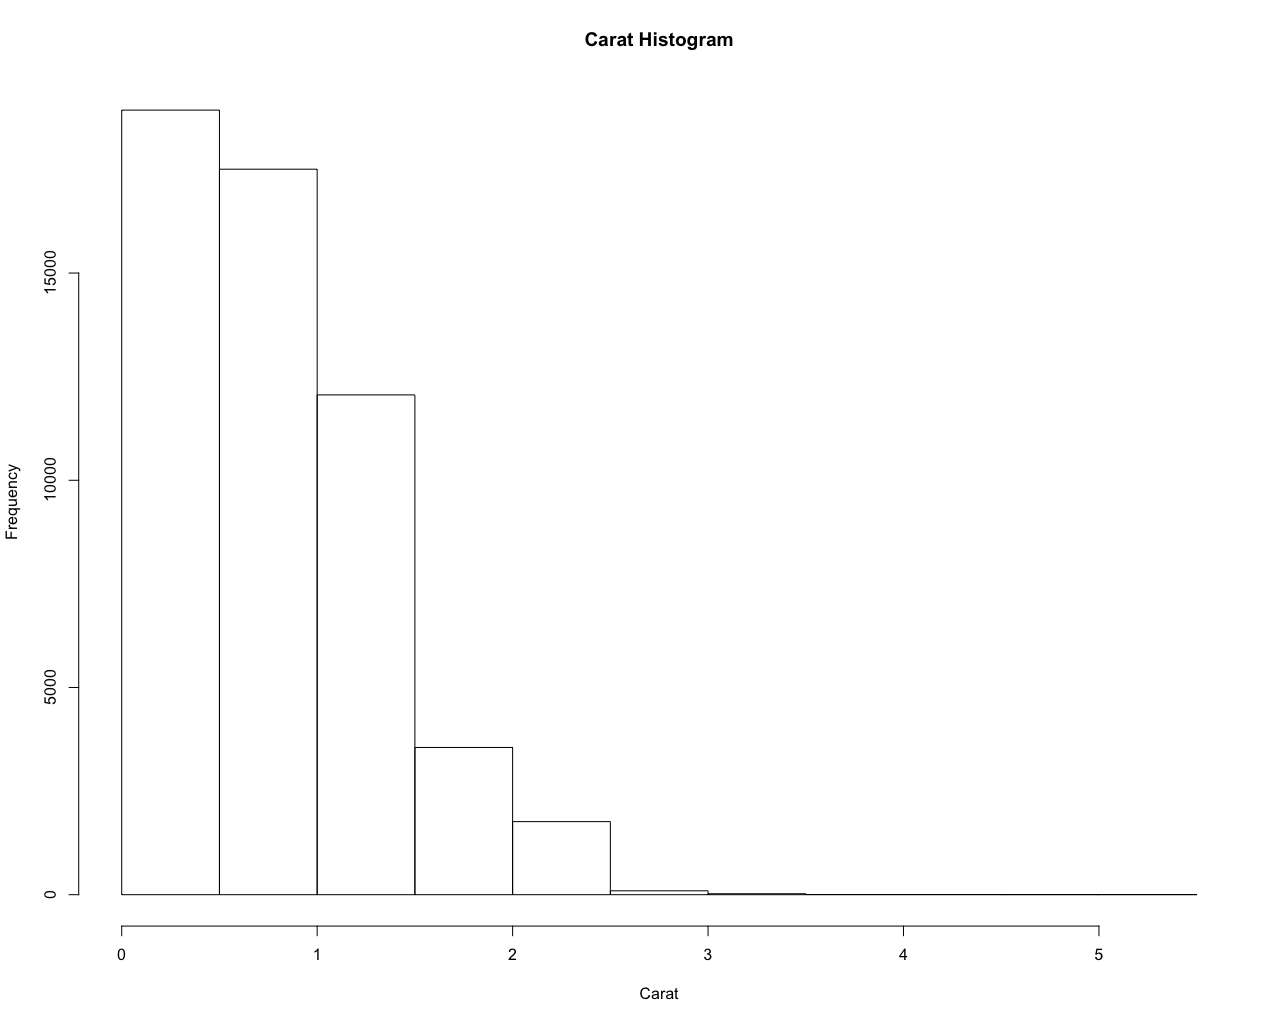
\includegraphics[width=1.0\linewidth]{pic0021}
  \caption{Хистограма на каратите}
\label{figure0021}
\end{figure}
\FloatBarrier

Хистограмата се изчислява като предварително се избират броят групи, в които да се класифицират стойностите (Листинг \ref{listing0069}), а след това се преброяват колко от стойностите попадат в съответната група.

\begin{lstlisting}[caption=Хистограма с повече групи, label=listing0069]
hist(diamonds$carat, main="Carat Histogram", xlab="Carat", nclass=100)
\end{lstlisting}

Функцията hist самостоятелно избира броят групи (nclass), но когато е нужна по-дребна гранулярност тя може да бъде изрично зададена (Фиг. \ref{figure0022}).

\begin{figure}[h!]
  \centering
  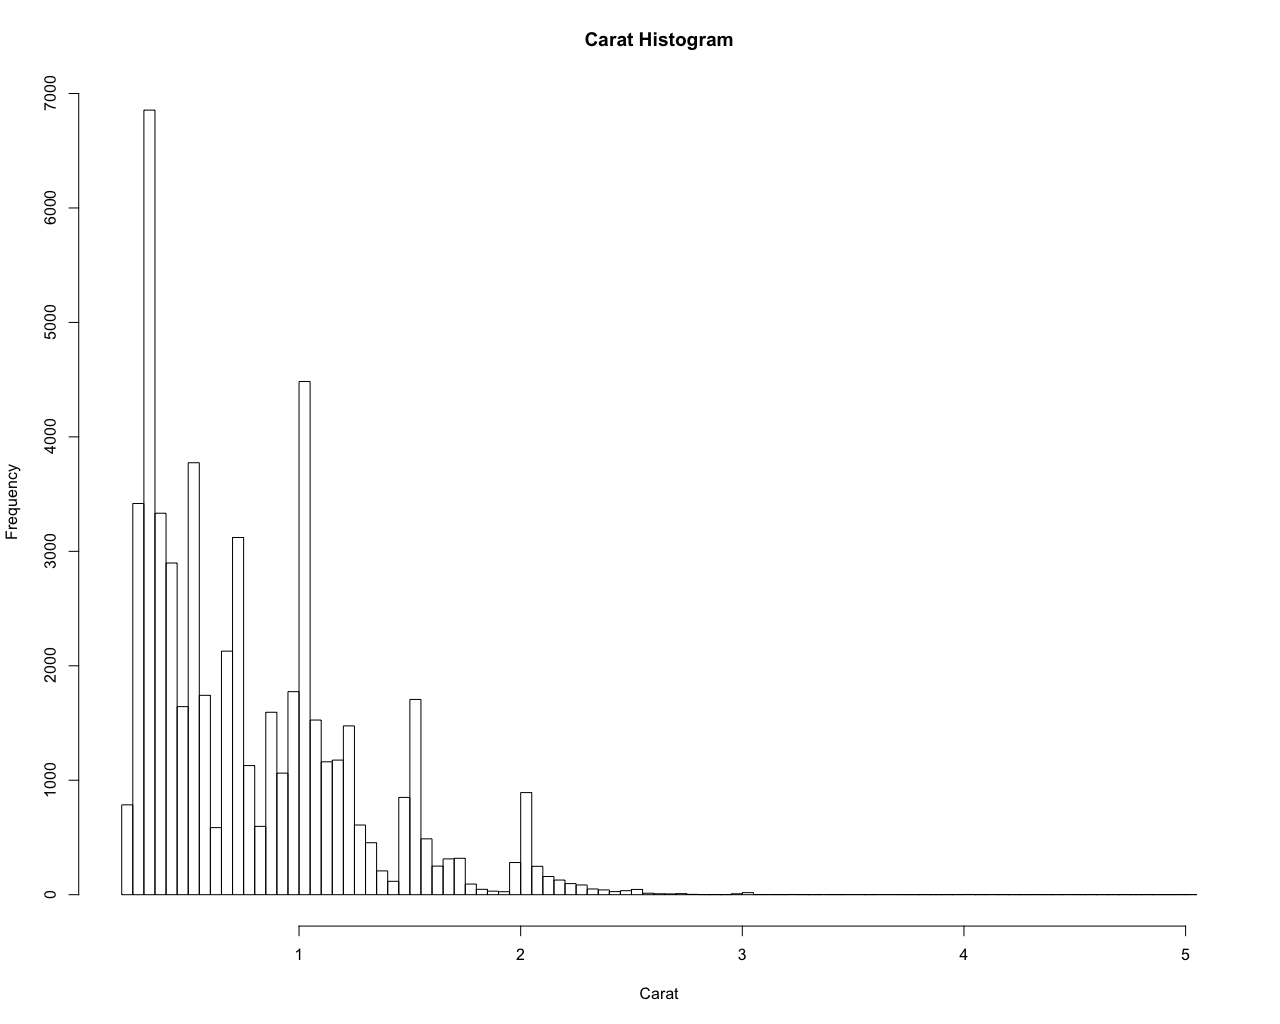
\includegraphics[width=1.0\linewidth]{pic0022}
  \caption{Хистограма на каратите при 100 групи}
\label{figure0022}
\end{figure}
\FloatBarrier

При изследването на непозната вероятностна променлива, хистограмата е първият инструмент, който може да послужи за ориентир какъв статистически анализ да се приложи. Колко групи да се използват за генериране на хистограмата, най-често се определя с експерименти, докато се достигне желаната експресивност.

\subsection{Диаграма на разсейване}

В статистическата обработка на данни много често е от значение как две случайни променливи си влияят една на друга. В такава ситуация изключително полезен инструмент се явява диаграмата на разсейване\index{диаграма на разсейване} (scatter plot). Всяка точка на диаграмата отразява едно наблюдение на двете променливи. Едната променлива се отчита по оста x, а другата променлива се отчита по оста y.

\begin{lstlisting}[caption=Генериране на диаграма на разсейване, label=listing0070]
plot(price~carat, data=diamonds)
\end{lstlisting}

Чисто интуитивно знаем, че колкото по-голям е един скъпоценен камък, толкова по-висока е цената му. В същото време, цената на камъка се определя и от други фактори. Диаграмата на разсейването (Листинг \ref{listing0070}) може да ни покаже каква е връзката между тегло и цена при скъпоценните камъни като не отчита другите фактори за определяне на цената.

\begin{figure}[h!]
  \centering
  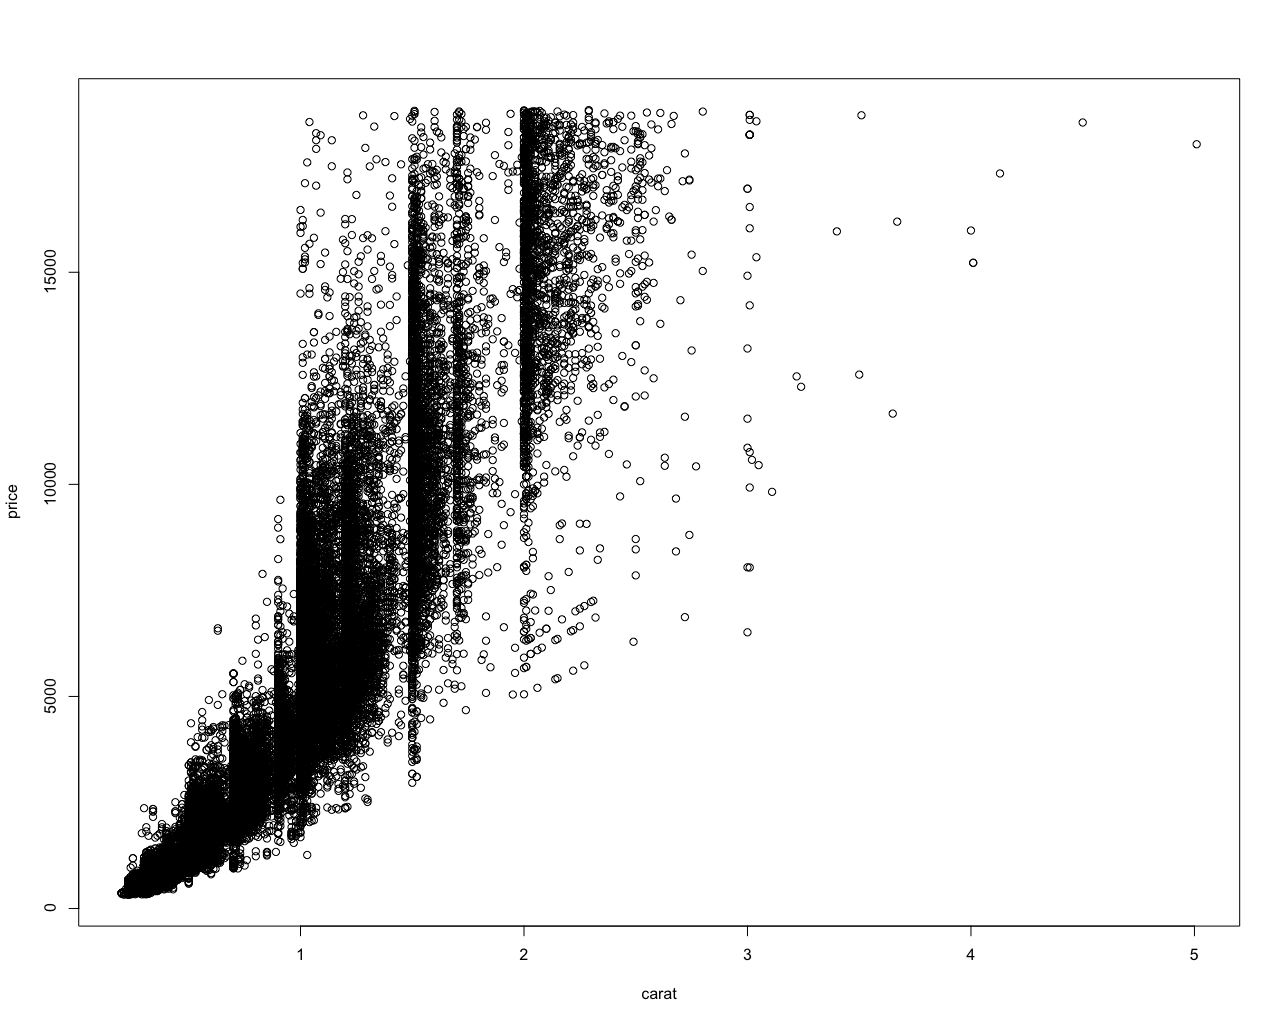
\includegraphics[width=1.0\linewidth]{pic0023}
  \caption{Диаграма на разсейване за камъните според отношението тегло към цена}
\label{figure0023}
\end{figure}
\FloatBarrier

За разчертаването на диаграмата се използва нотацията за формули. При тази нотация, символът тилда (\textasciitilde) показва, че се търси зависимостта  на цената от теглото. Поради тази причина цената се изобразява на ординатната ос, а теглото на камъка на абсцисната ос. На Фиг. \ref{figure0023} ясно се вижда, че с нарастване на размера, нараства и цената на скъпоценния камък. В допълнение се забелязват и някои по-особени зони, които нарушават равномерното разпределение на точките. Този вид аномалии подсказват за наличието и на други фактори при формирането на цената. Тъй като информацията е недостатъчна, диаграмата на разсейването не може да даде идея кои фактори допълнително оказват влияние за образуването на цената.

\begin{lstlisting}[caption=Алтернативна команда за диаграма на разсейване, label=listing0071]
plot(diamonds$carat, diamonds$price)
\end{lstlisting}

Не е нужно вероятностните променливи да се намират в един data.frama за да се генерира диаграма на разсейване. Достатъчно е да се използва алтернативния запис за извикване на функцията plot (Листинг \ref{listing0071}).

\subsection{Графики тип кутия}

Графиките тип кутия\index{графика тип кутия} (box plot) са инструмент за изобразяване на статистическа информация, който не среща голямо одобрение в общността на статистиците. Въпреки мнението в професионалните общности, графиките тип кутия са често използвани от студентите.

\begin{lstlisting}[caption=Генериране на графика от тип кутия, label=listing0072]
boxplot( diamonds$carat )
\end{lstlisting}

Информацията от хистограмата за каратите на скъпоценните камъни може да се представи в значително по-стилизиран вид, чрез графики от тип кутия (Листинг \ref{listing0072}).

\begin{figure}[h!]
  \centering
  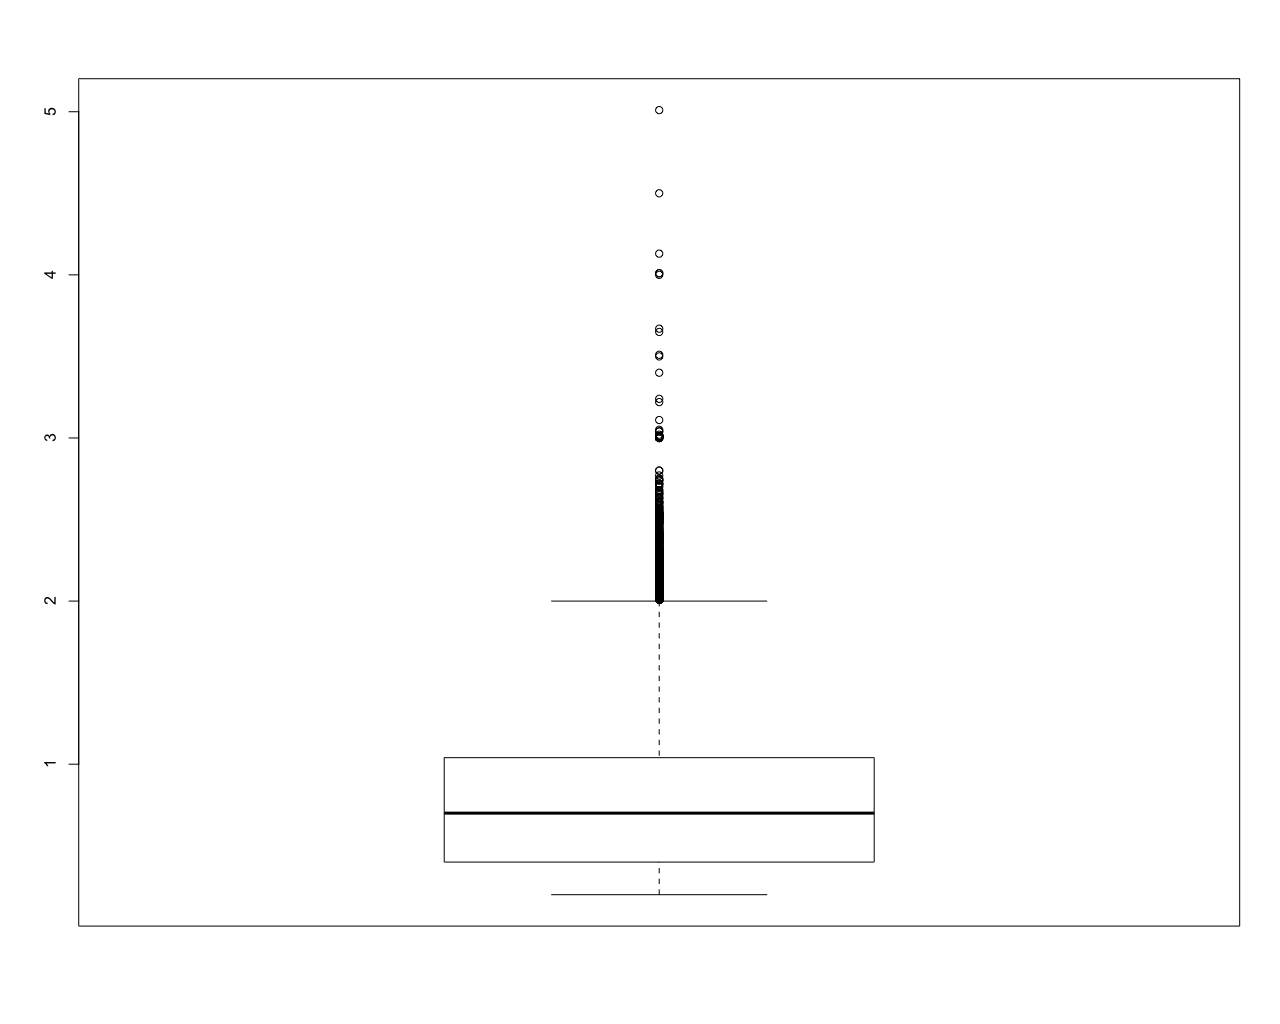
\includegraphics[width=1.0\linewidth]{pic0024}
  \caption{Графика тип кутия за теглото на диамантите}
\label{figure0024}
\end{figure}
\FloatBarrier

При графиката от тип кутия (Фиг. \ref{figure0024}) линията, която преминава през средата на кутията показва къде е медианата на множеството от стойностите. Медианата се изчислява като се сортират всички елементи и се вземе стойността на елемента, който стои в средата. Ако броят елементи е четно число, медианата е средна стойност между двете стойности, стоящи в средата на множеството. Медианата разделя множеството на две равни части. Горният и долният ръб на кутията показват първия квартил и третия квартил. На практика, тези три черти разделят множеството от стойности на четири равни части. При графиките от тип кутия понякога се получава нещо наречено опашка и се изобразява с точки от единични измервания. Тези стойности се смятат твърде необичайни и е прието да се изпускат в определянето на параметрите за кутията. В най-долния и най-горния край са отчетени най-малкият карат и най-големият карат в примерното множество от данни.

Графиките от тип кутия често се използват при изследвания с Монте Карло симулации\index{Монте Карло симулации}, където трябва да се демонстрира сходимостта на стохастичния процес. От практиката е наложено да се правят 30 измервания по оста на времето и обобщената статистика за всяко измерване да се визуализира под формата на графика тип кутия.

\section*{Заключение}

Коректното въвеждане на данните в системата е от изключителна важност за осъществяването на коректен анализ и постигането на приемливи статистически резултати. В другия край на процеса е самото визуализиране на получените резултати и максималната експресивност, която може да се постигне за представянето пред широка аудитория. Тези две стъпки от процеса по статистически анализ са свързани с въвеждането на информацията и графичното визуализиране на получените резултати.

